\documentclass[12pt]{article}
\usepackage{parskip}
\usepackage[letterpaper, margin=1in]{geometry}
\usepackage{graphicx}
\usepackage{amsmath}
\usepackage{pdflscape}
\usepackage{tikz}
\usepackage{fancyhdr}
\renewcommand{\headrulewidth}{0pt}
\usepackage{titlesec}
\fancypagestyle{lscapedplain}{%
  \fancyhf{}
  \fancyfoot{%
    \tikz[remember picture,overlay]
      \node[outer sep=1cm,above,rotate=90] at (current page.east) {\thepage};}
}
\graphicspath{{./images/}}
\title{ELECENG 2EI5 Project 2}
\author{Raeed Hassan \\ hassam41 \\  \\ McMaster University}
\begin{document}
\maketitle
\pagebreak

\begin{enumerate}
    \item An ideal switch should function as an open circuit when it is open and function as a short circuit when it is closed. When the switch is open, there should be no current through the switch. When the switch is closed, the voltage on both terminals of the switch should be the same.
    \item %The circuit topology that you selected for each type of switch.
    The circuit topology used for switch 1 is simply a p-channel MOSFET in enhancement mode. $V_{control}$ is the gate voltage, while $v_1$ and $v_2$ are the source and drain of the MOSFET. This design was chosen because it was the only design I discovered that could be built with the components outlined in the design constraints.

    The circuit topology used for switch 2 is two MOSFETS, one n-channel and one p-channel. The gates of both MOSFETS are connected to $V_control$. Their sources connected to the $V_A$ and $V_B$, while their drains are connected to the same node, with the node also connecting a resistor to ground. This design was chosen because it was the only design I discovered that could be built with the components outlined in the design constraints.
    \item %The main non-idealities that your design has. For each non-ideality:
    In switch 1, there are 3 non-idealities present. These are the voltage drop across the MOSFET when the switch is closed, the current through the MOSFET when the switch is open and the operating range for $v_1$.

    In switch 2, there are 2- non-idealities present. These are the voltage drop across the two MOSFETS when the two oterminals are expected to have the same voltage and the operating range for $V_A$ and $V_B$.
    \begin{enumerate}
        \item %Justify using a design that has this non‐ideality .I.e. explain benefit of using this design despite this particular non‐ideality instead of alternate designs.
        In general, with the use of real components, there will almost always be some sort of voltage drop across the component and some current flowing through the current. This non-idealities are unavoidable, therefore the focus should be on minimizing them when relevant. The design chosen will perform relatively well despite these two non-idealities because the presence of a large resistor in the drain will both decrease the voltage drop when the switch is closed and decrease the current through the MOSFET when the switch is open, and this has been confirmed in simulations. The possible operating range for $v_1$ is also not a large issue as long as the circuit works at a reasonable range. The operating range for $v_1$ can just be taken as a given for the circuit, similar to how many electronic devices have specified voltage ranges for them to function.

        In general, there will always be a voltage drop across the two MOSFETS when ideally there should be no drop across the terminals of the MOSFET when the MOSFET is in cutoff. This non-ideality is unavoidable, however the design should still perform relatively well due the presence of a large resistor in the drains of the MOSFETS, minimizing the voltage drop across the MOSFET. The possible operating ranges for $V_A$ and $V_B$ would generally not be a large issue if they were specificied, however this cannot be tested due to the large number of possible combinations of $V_A$ and $V_B$.  
        \item %Quantify the performance of your design in theory.
        In theory, the switch should have a slight voltage drop across the MOSFET when it is closed, which means that $v_1 \neq v_2$. When the switch is open, there should be very little current through the MOSFET, this means $i_D$ is near 0.

        In theory, the $v$ should be slightly less than $V_A$ when $V_{control} = 0$ and $v$ should be slightly less than $V_B$ when $V_{control} = 5$.
        \item %Specify how you can measure the performance of your design.
        The performance of switch 1 can be measured in both the open and closed state by measuring how close the real values are to their intended values. This means we can test the voltage drop across the MOSFET, $v_1-v_2$, when the switch is closed and we can test the current through the MOSFET, $i_D$, when the switch is open. We can also evaluate the voltage range for $v_1$ for which the switch functions.

        The performance of switch 2 can be measured by measuring the voltage at $v$ and comparing it to its intended voltage ($V_A$ or $V_B$) depending on $V_{control}$. The difference between $v$ and the input voltage can be used to measure the performance of the switch. The operating voltage ranges for $V_A$ and $V_B$ can also be tested, however they are not tested in this experiment due to the difficulty of testing all possible combinations of the two voltages.
    \end{enumerate}
    \item Simulations
    \begin{enumerate}
        \item %What simulations did you choose to perform?
        Two simulations were run for switch 1. One simulation measured the voltage drop across the p-channel MOSFET when $V_{control}$ was 0V (the switch should be closed). The other simulation measured the current $i_D$ by measuring the current through the resistor when the switch was open ($V_{control} = 5V$). Both simulations were transient analyses with a stop time of 5ms.

        For switch 2, the only simulation ran measured the in the node connected to the drains of the two MOSFETS. This was a transient analyses with a stop time of 5ms.
        \item %What Spice models did you have to use and how did you obtain parameters for those models?
        The p-channel and n-channel MOSFETS used for the simulation of switch 1 and 2 was the general p-channel and n-channel MOSFET models provided in the general LTSpice library. The manufacturer of the MOSFET does not provide a spice model for the component or the necessary parameters needed to model the the MOSFET, therefore I used the default MOSFET model, accepting that it would have different parameters than the built circuit.
    \end{enumerate}
    \item Measurement
    \begin{enumerate}
        \item %What are the important specifications of your design?
        The most important specifications for switch 1 were the voltage drop across the MOSFET when the switch was closed (very close to 0V), the current through the MOSFET when the switch was open (very close to 0A), and the operating ranges of $v_1$ where the switch functioned (2-5V when the switch is closed, 0-5V when the switch is open).
        
        The most important specification for switch 2 is the voltage $v$ at both control voltages ($V_{control} = 0V$ and $V_{control} = 5V$).
        \item %Using your test plan (items mentioned in 1c above) report measurements on your circuit and compare the results with what you expected from hand calculations and Spice simulations.
        The results for switch 1 was matched the expectations that were determined from the general theory of a MOSFET and our simulationss. Due to the presence of a large resistor at the source, the voltage drop when the switch was open and the current when the switch was closed was largely negible, meeting the specifications of the switch. One discrepancy between the results and the simulations was the operating range for $v_1$ when the switch was open, however this could be expected the as spice model used for simulations likely had a value of zero for $V_T$ while our MOSFET had a non-zero value. This would have limited the operation range of the MOSFET when the source voltage $v_1$, did not have a large enough difference from the gate voltage.

        The circuit for switch 2 was not built.
    \end{enumerate}
\end{enumerate}
\pagebreak
\begin{landscape}
    \pagestyle{lscapedplain}
    \appendix
    \section{Figures - Switch 1}
    \begin{figure}[ht!]
        \begin{minipage}[b]{0.33\linewidth}
            \centering
            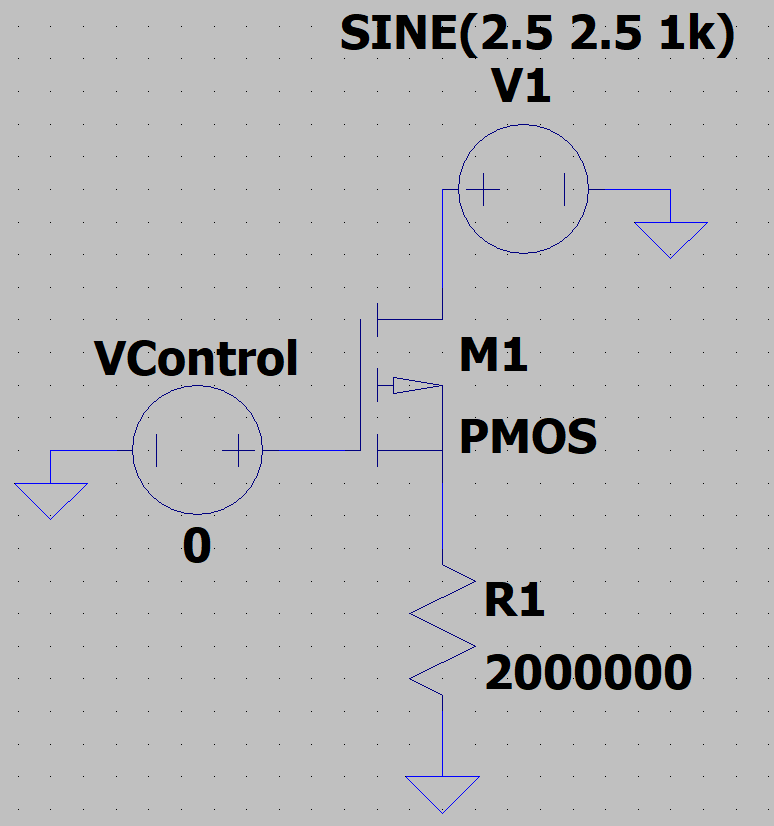
\includegraphics[width=0.7\linewidth]{images/S1Schematic.png} 
            \caption{Schematic of switch 1} 
            \vspace{4ex}
        \end{minipage}%%
        ~
        \begin{minipage}[b]{0.33\linewidth}
            \centering
            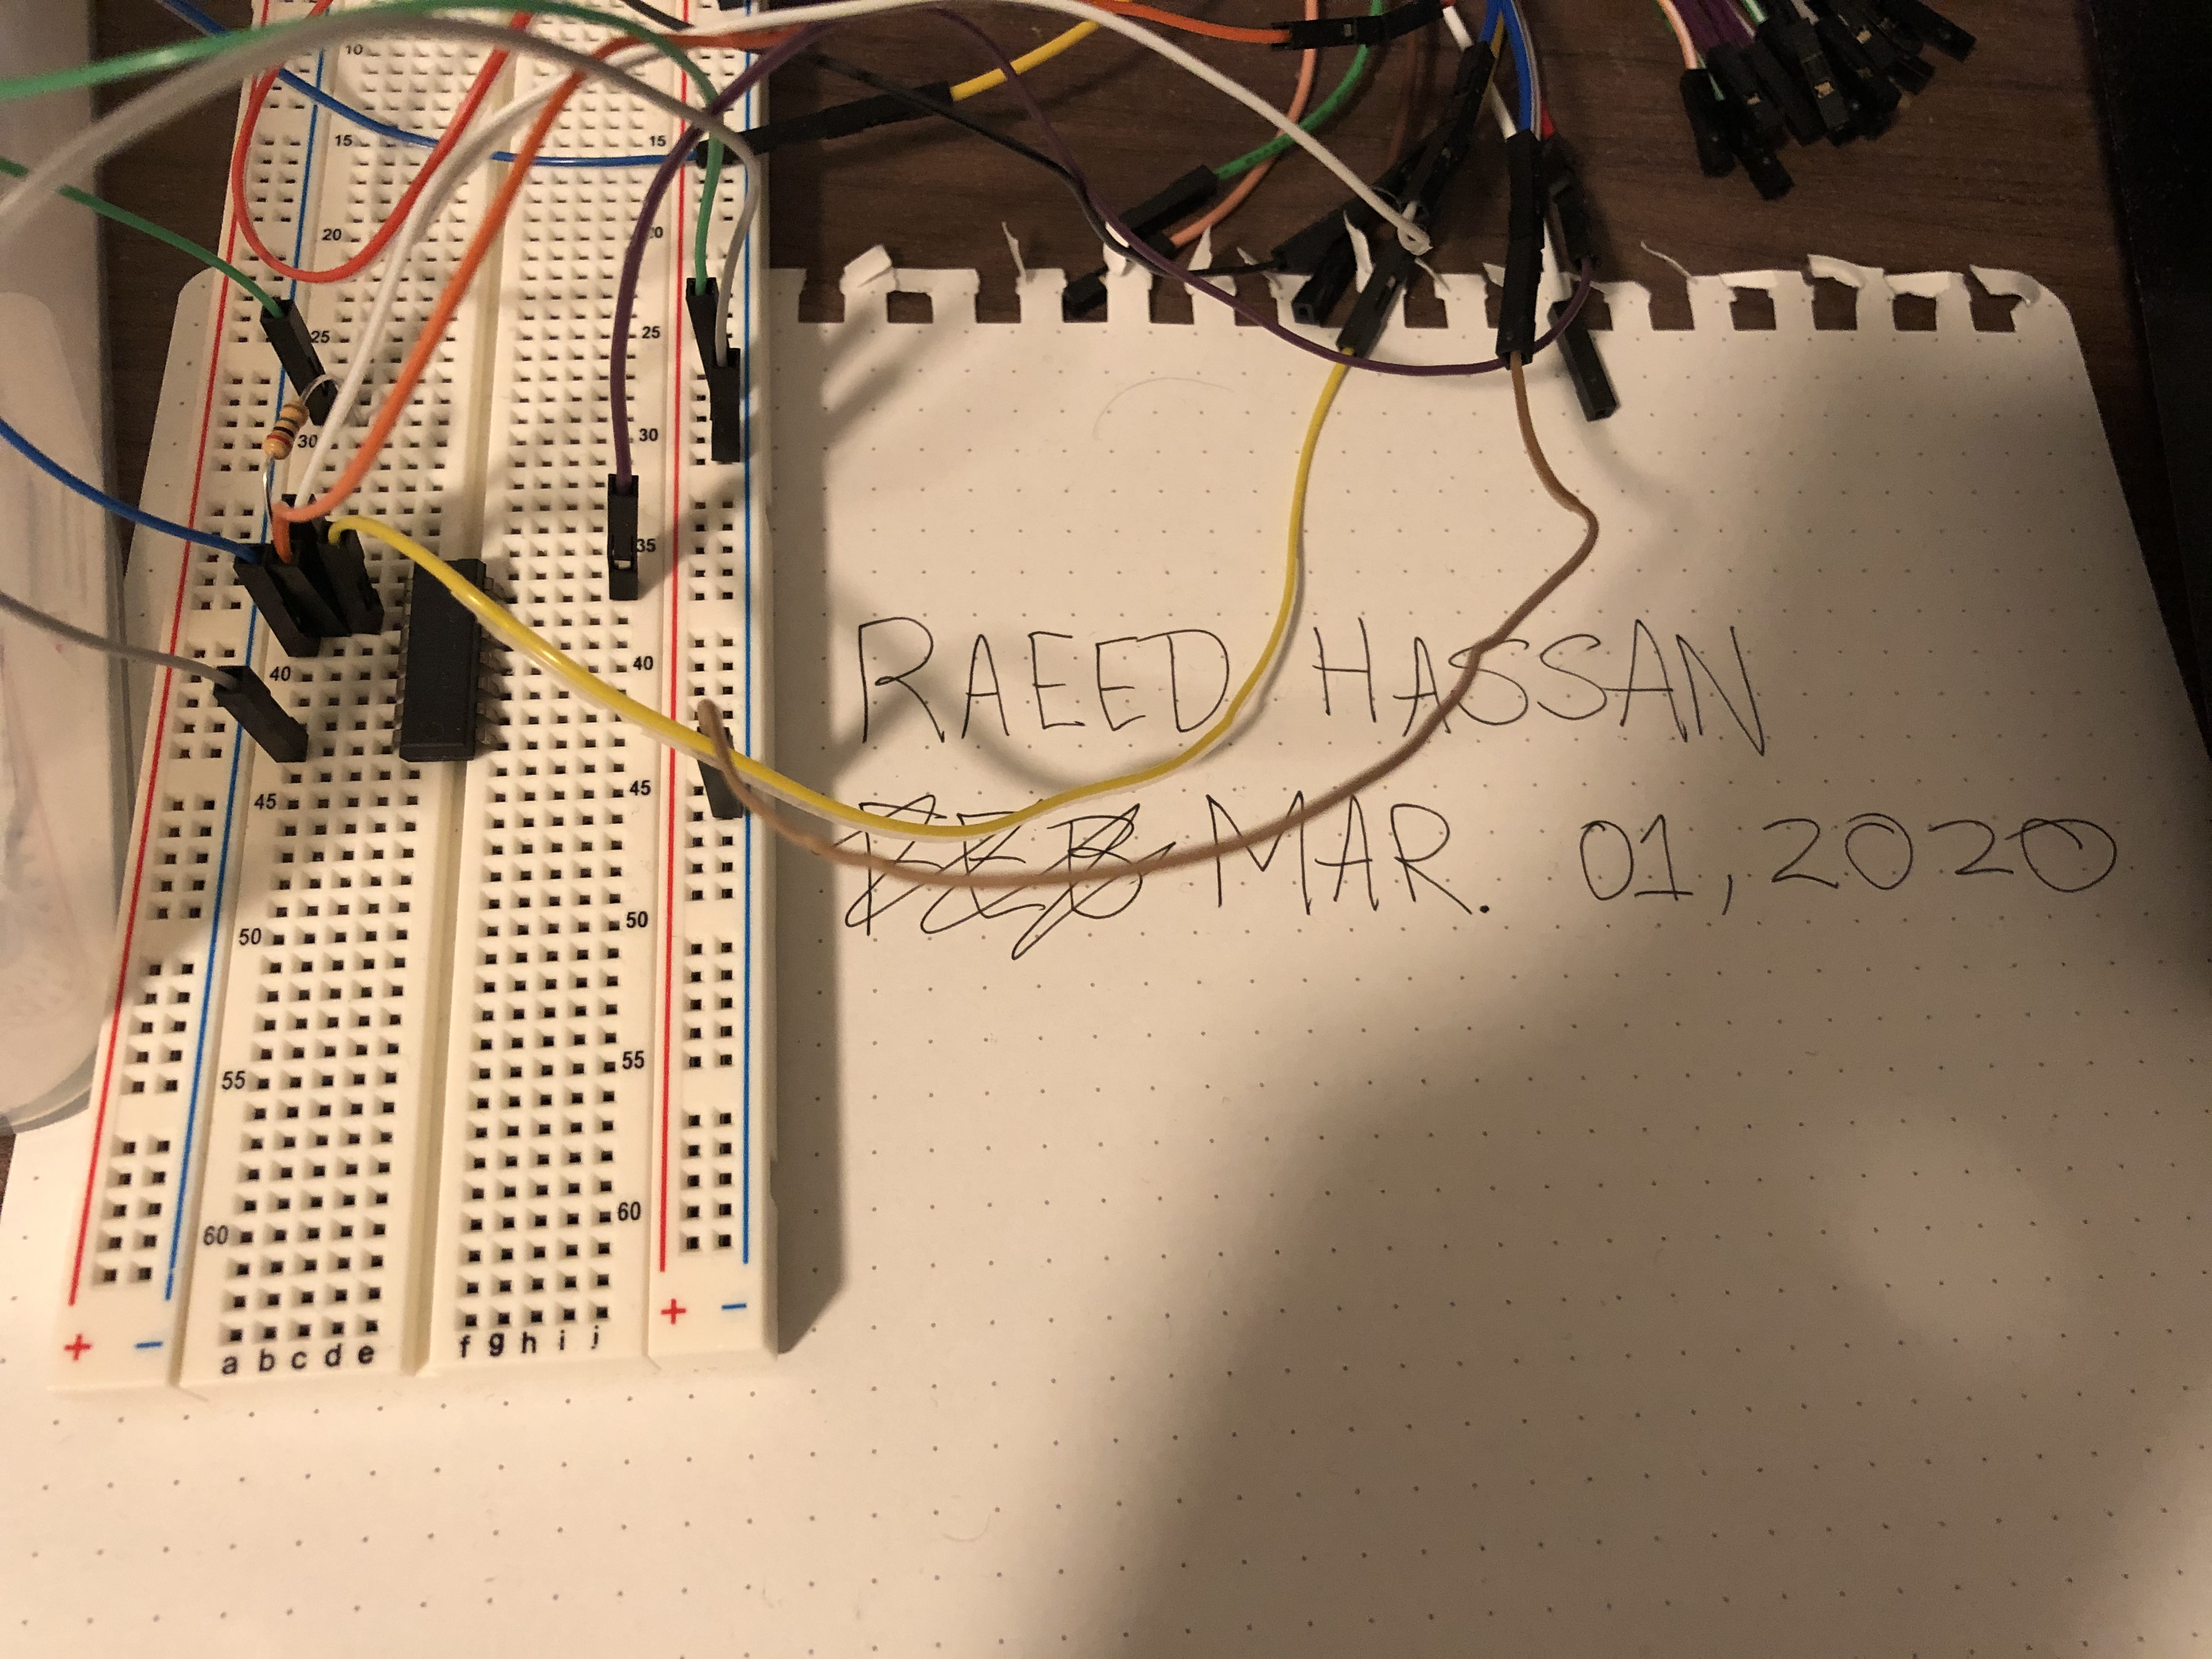
\includegraphics[width=\linewidth]{images/Switch1Circuit.png} 
            \caption{Circuit of switch 1} 
            \vspace{4ex}
        \end{minipage}%%
        ~
        \begin{minipage}[b]{0.33\linewidth}
            \centering
            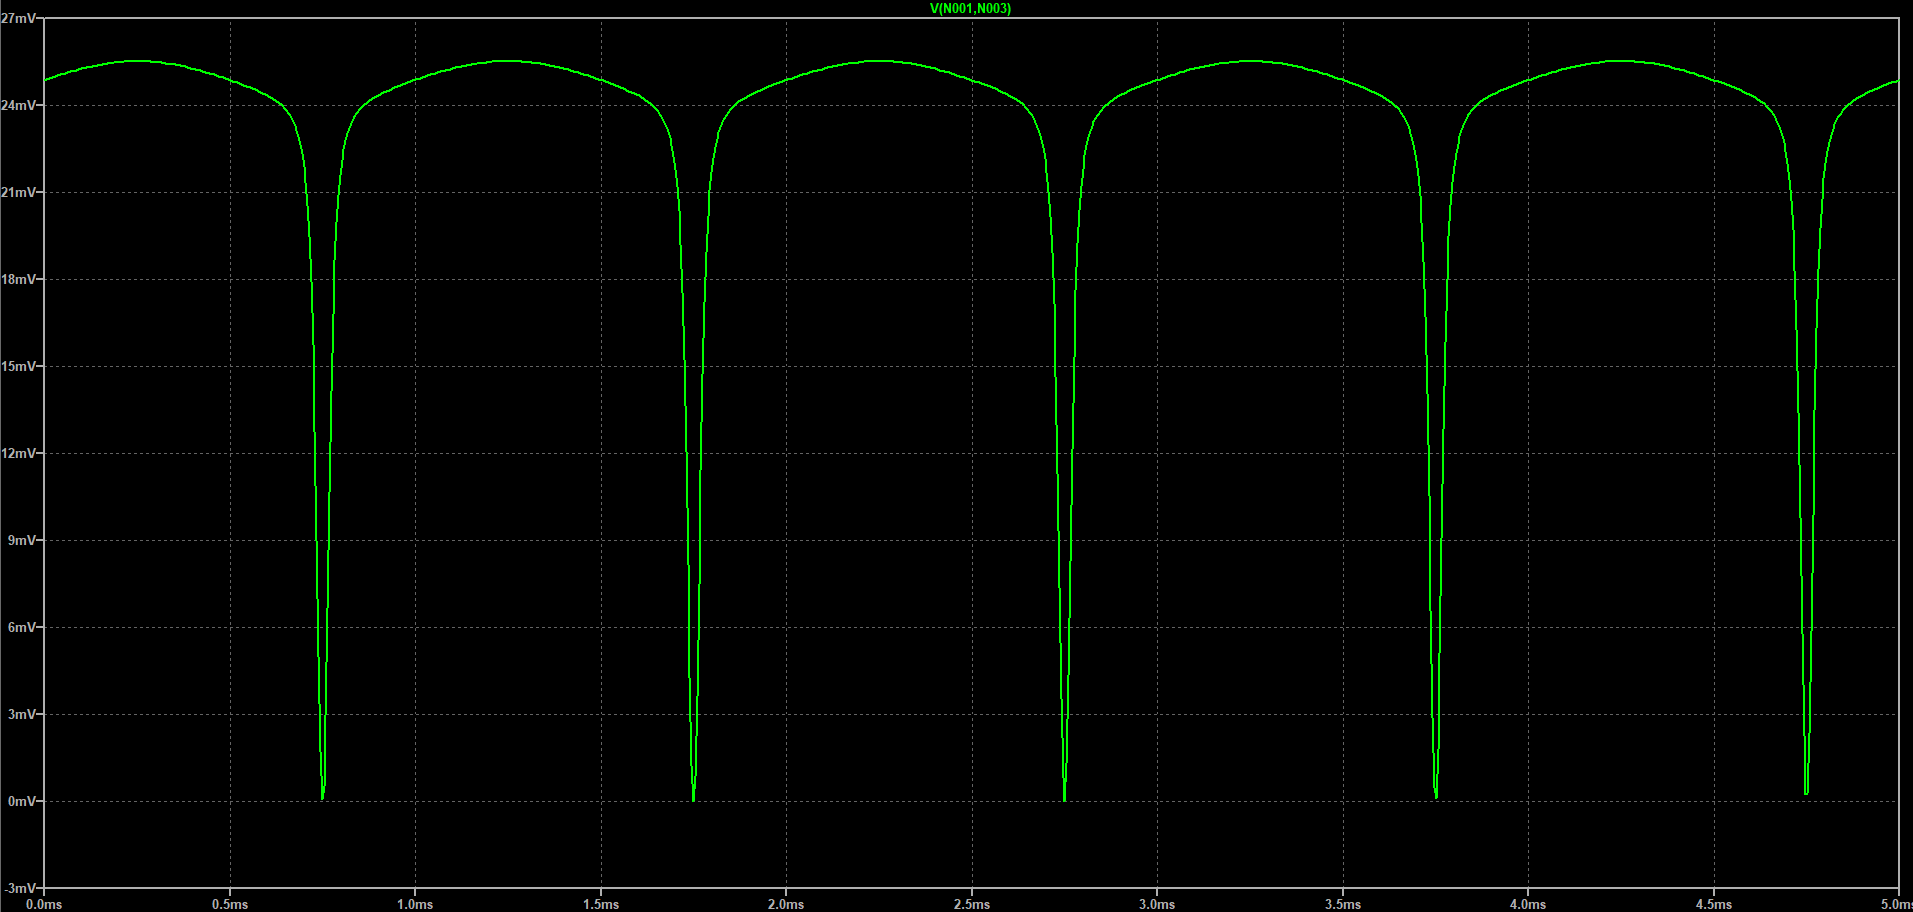
\includegraphics[width=\linewidth]{images/S1ClosedSim.png} 
            \caption{Simulated MOSFET voltage drop (closed)} 
            \vspace{4ex}
        \end{minipage}
        \begin{minipage}[b]{0.33\linewidth}
            \centering
            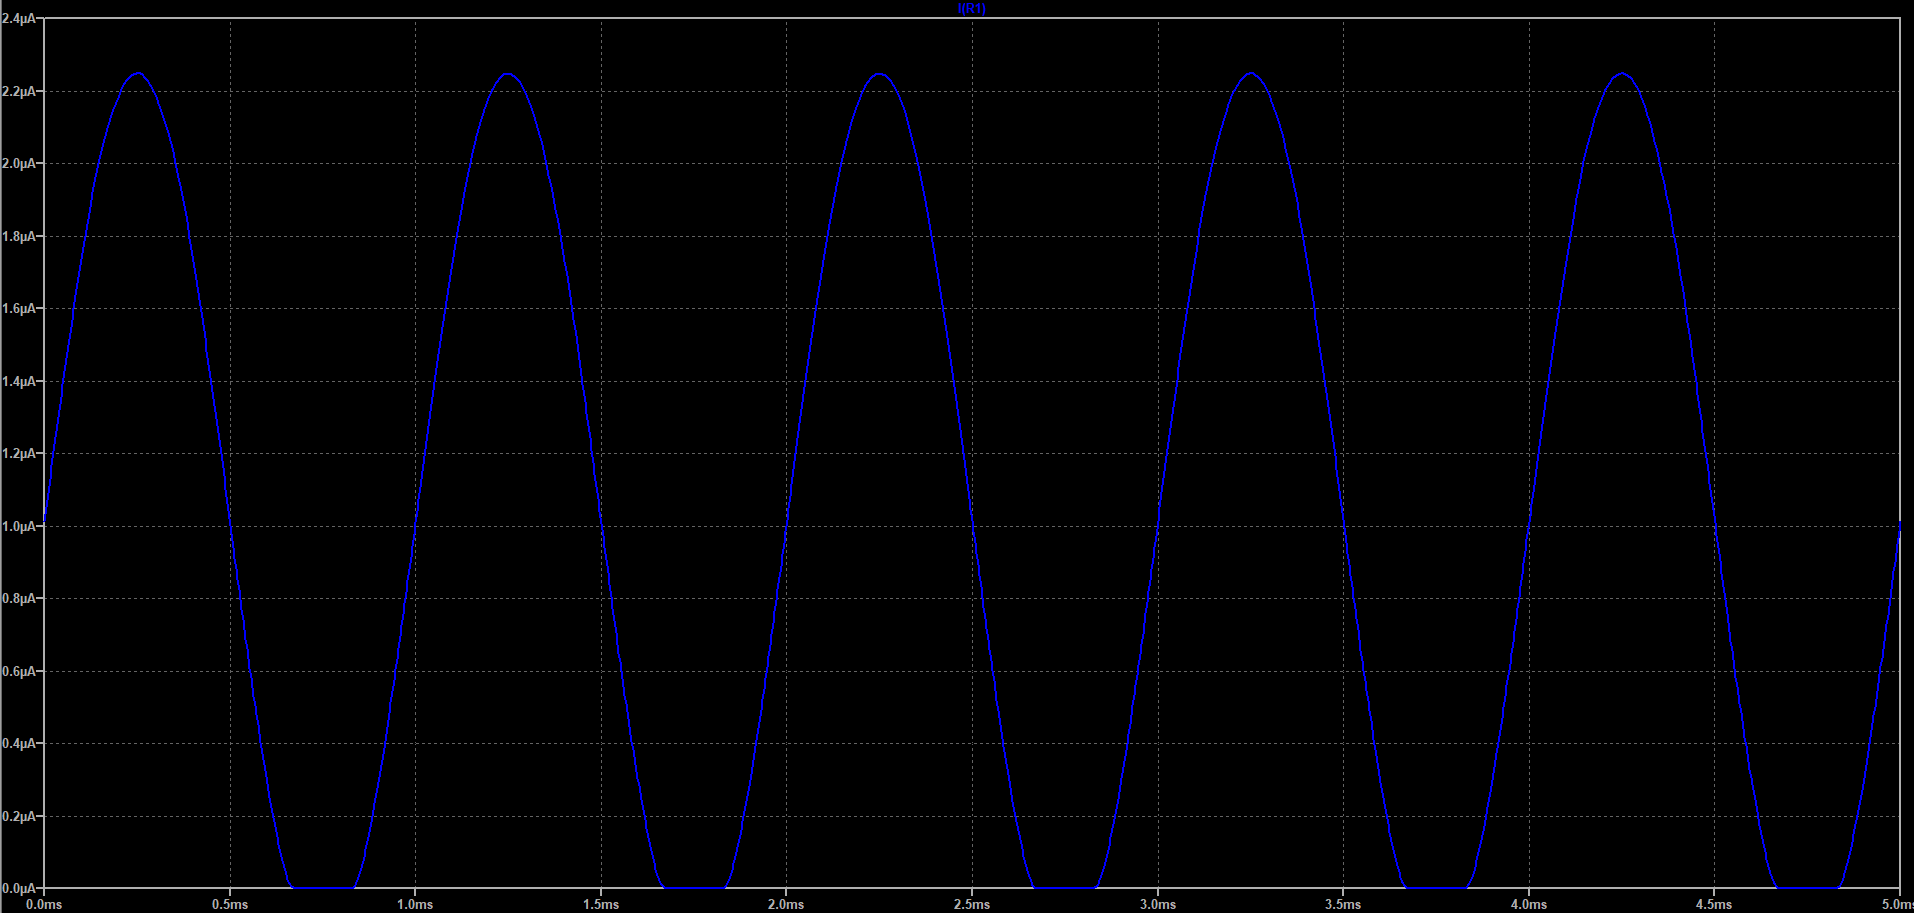
\includegraphics[width=\linewidth]{images/S1OpenSim.png} 
            \caption{Simulated current through MOSFET (open)} 
            \vspace{4ex}
        \end{minipage}%%
        ~
        \begin{minipage}[b]{0.33\linewidth}
            \centering
            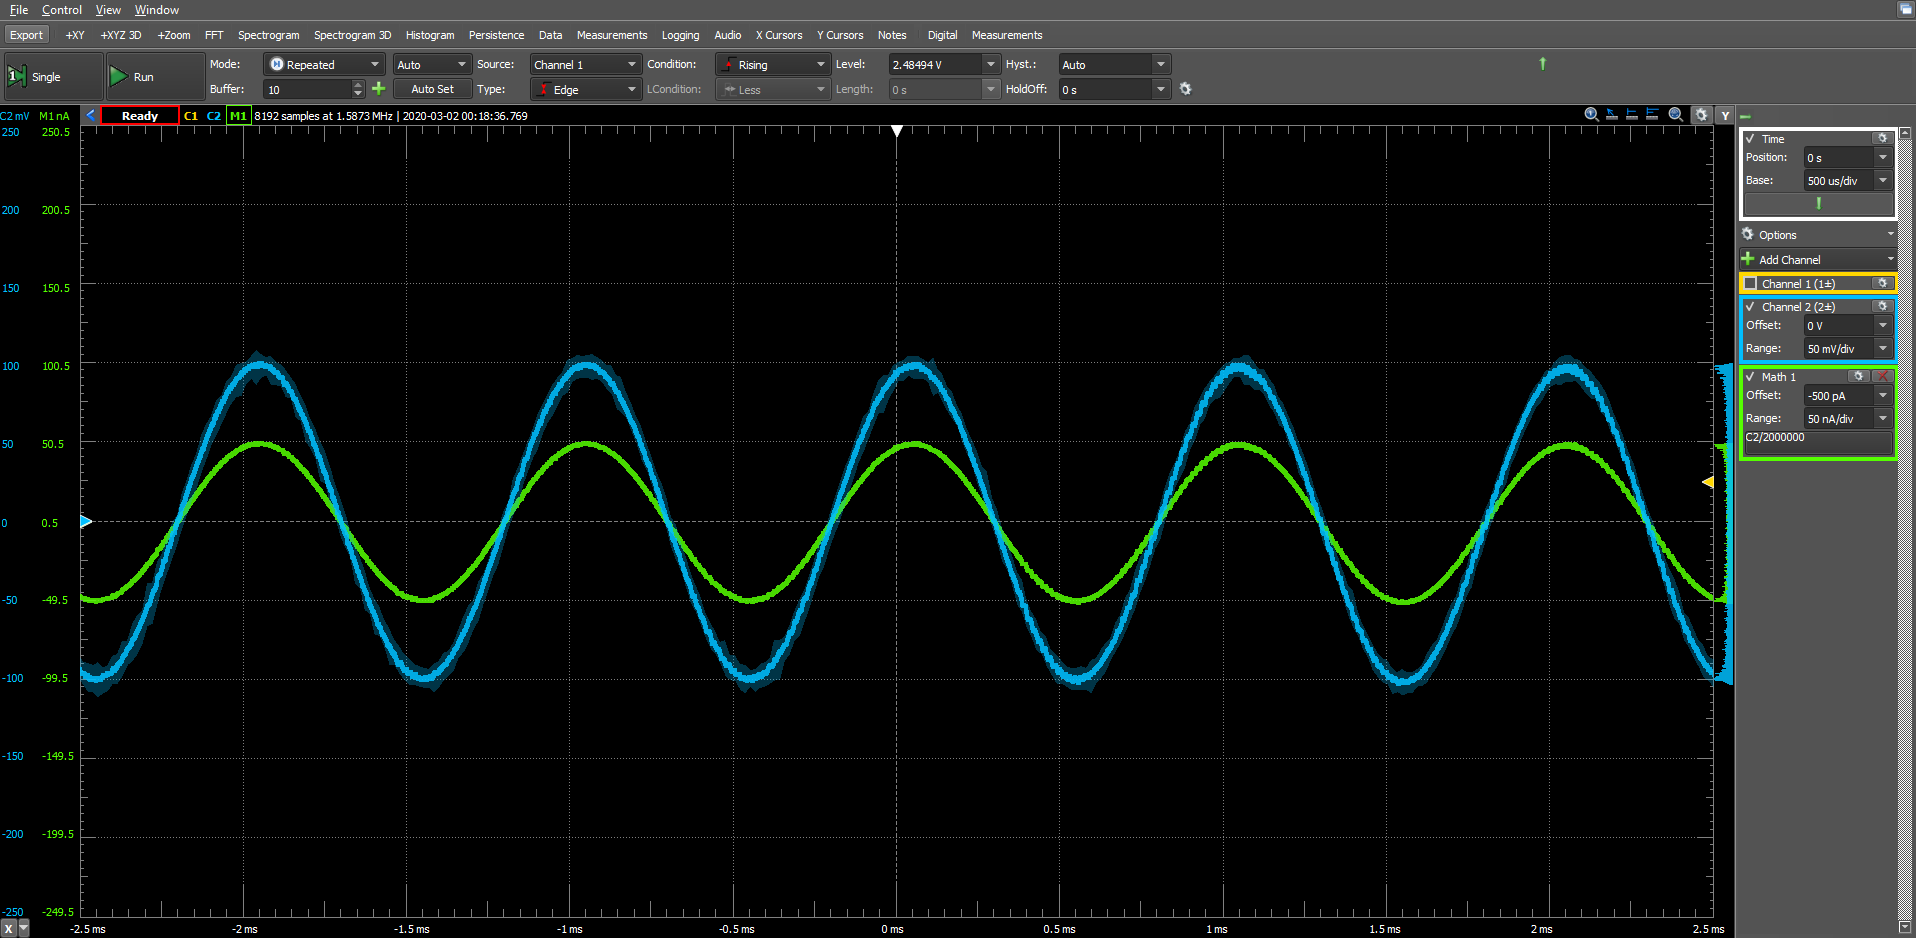
\includegraphics[width=\linewidth]{images/S1Open.png} 
            \caption{Measured current through MOSFET (open)} 
            \vspace{4ex}
        \end{minipage}%%
        ~
        \begin{minipage}[b]{0.33\linewidth}
            \centering
            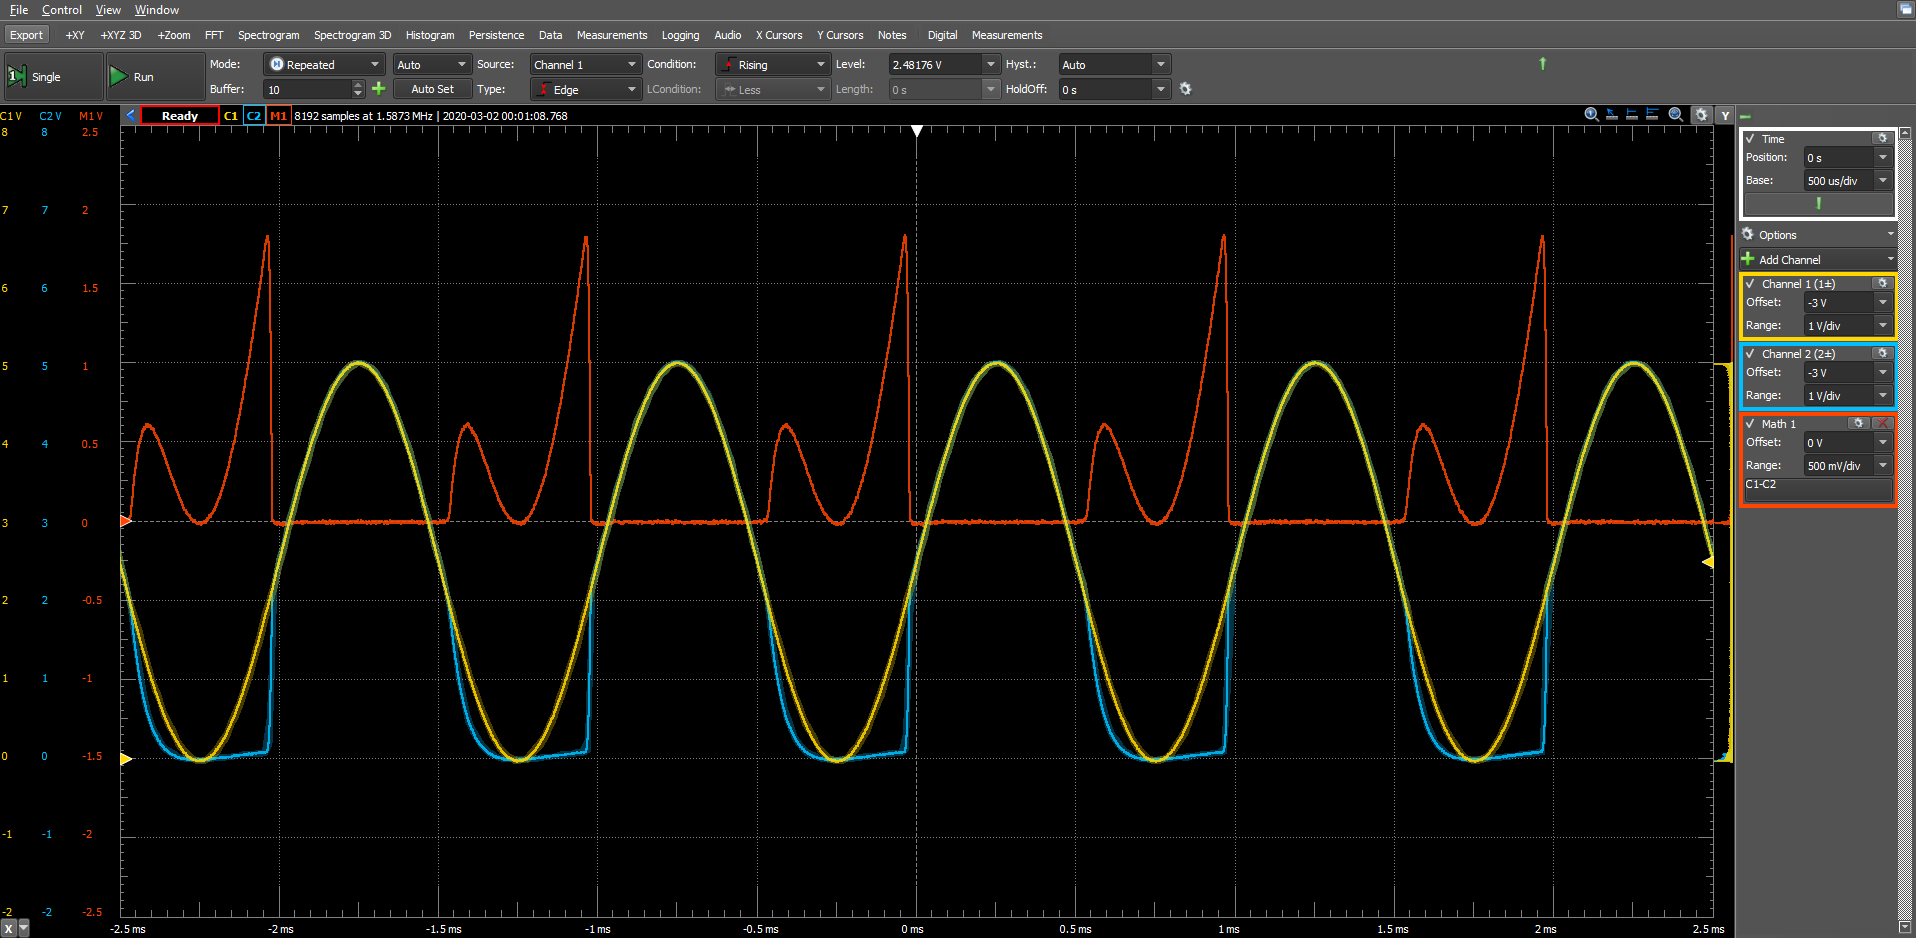
\includegraphics[width=\linewidth]{images/S1Closed.png} 
            \caption{Measured MOSFET voltage drop (closed)} 
            \vspace{4ex}
        \end{minipage}%%
    \end{figure}
\end{landscape}
\pagebreak
\begin{landscape}
    \pagestyle{lscapedplain}
    \appendix
    \section{Figures - Switch 2}
    \begin{figure}[ht!]
        \begin{minipage}[b]{0.33\linewidth}
            \centering
            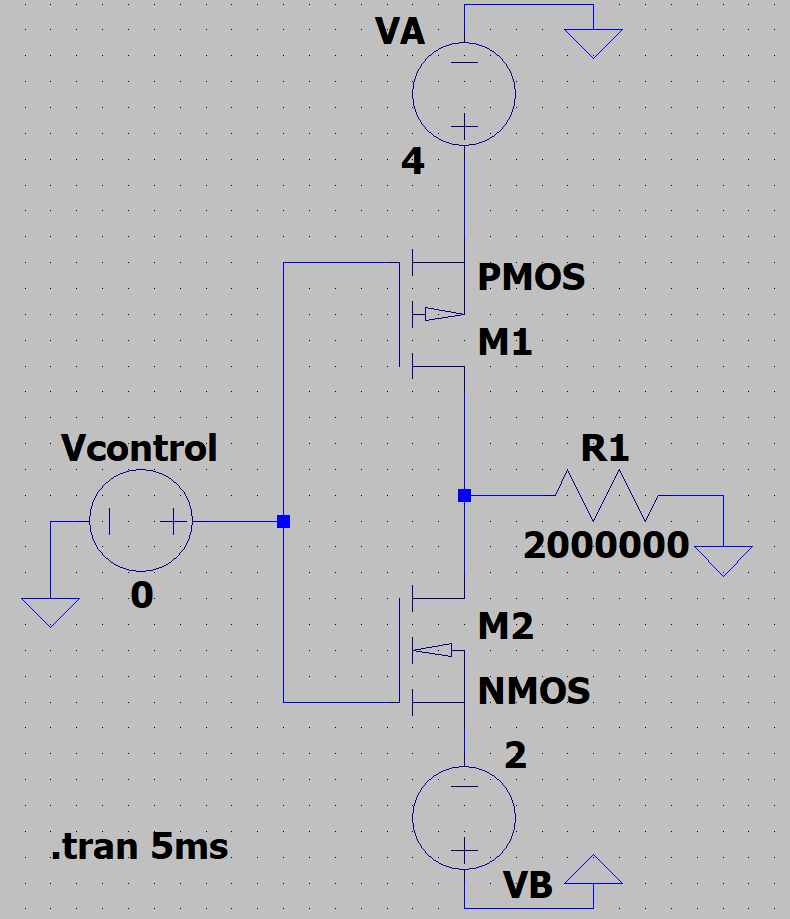
\includegraphics[width=0.7\linewidth]{images/S2Schematic.png} 
            \caption{Schematic of switch 2} 
            \vspace{4ex}
        \end{minipage}%%
    \end{figure}
\end{landscape}
\end{document}